\documentclass[12pt, oneside]{article}   
\usepackage{textcomp}

\usepackage{listings}
\lstset{language=R,literate={<-}{{$\gets$}}1}

\usepackage[a4paper,bindingoffset=0.2in,%
            left=0.75 in,right= 0.75 in,top= 0.75 in,bottom=0.75in,%
            footskip=.55in]{geometry}

                		
\geometry{letterpaper}                   		
\usepackage{amsmath}
\usepackage{graphicx}

\setlength{\parindent}{0pt}

\title{Bayesian Analysis of Randomized Controlled Trials}
\author{Julian Bautista, Alex Pavlakis, Advait Rajagopal}
%\date{\today}		
			
\begin{document}
\maketitle

\abstract{}	

\newpage 

\tableofcontents
\newpage

\section{Introduction}
Bayesian methods are gaining popularity in many fields because they allow researchers to incorporate all available information into flexible and transparent statistical models.  Many researchers have begun to incorporate Bayesian methods into medical, pharmaceutical, and social-science research.  The purpose of this paper is to show how Bayesian methods can be the standard in applied research.  We provide a general overview of the approach and an example analysis of Randomized Control Trial (RCT) on the impact of a smartphone application on eating disorder behavior.  

\section{Bayesian Data Analysis}
Bayesian data analysis (BDA) and inference is the process of developing and fitting a probability model to data. The result is learning the probability distribution of the parameters of the model and being able to evaluate the fit of the model to the data as well being able to make predictions for new observations [Gelman et. al 2013; Gelman and Hill 2007].\\
There are three main steps to BDA and these are listed below and explained in detail in section 2.1, 2.2 and 2.3 respectively.
\begin{enumerate}
\item{Set up a probability model.}
\item{Calculate the distribution of the model parameters, given the observed data. This is called the \textit{posterior distribution} of the parameters.}
\item{Check the fit of the model, whether the conclusions are sensible and how sensitive they are to modeling assumptions. Expand or alter the model if needed and repeat the steps.}
\end{enumerate}

\subsection{Model development}
Developing a probability model means setting up a joint probability distribution in a way that it takes into account all observed data and unobserved quantities. It should include all knowledge of the experiment or data collection process and should be logically consistent with scientific nature of the problem at hand. This involves a \textit{prior distribution} and a \textit{likelihood function}.\\
 Bayesian analysis requires the assignment of a prior distribution that can restrict the set of values that a coefficient or parameter can take. This prior distribution also allows us to make our assumptions about the experiment and actual nature of the problem explicit. For example, if we were dealing with a regression prediction problem, we could assign a completely ``noninformative" prior to our coefficient which is equivalent to saying that the coefficient is a draw from a uniform distribution on the whole real line and moreover that all those values are equally likely. Incidentally this boils down to a maximum likelihood estimate of the coefficient. But statisticians are rarely in a position where they know absolutely nothing about the nature of their model parameters. Perhaps they know it needs to be positive, or, if what is being modeled is a probability then it needs to be between zero and one. Either way, this knowledge about the parameter should be made explicit and incorporated into the problem using an ``informative" prior distribution. In section 3 we discuss some advantages and choices of prior distributions. The likelihood function is the probability distribution of the observed data conditional on the parameters. Again, in a regression problem context, the likelihood function is a Gaussian distribution.\\
The Bayesian approach combines data and prior information, which coupled with the correct model yield more precise inferences than we could get from either source on its own.

\subsection{Model estimation}
The goal of model estimation is to calculate the \textit{posterior distribution} of the parameters. This is the conditional distribution of the parameter given the observed data. The posterior distribution is obtained by simply multiplying the prior and likelihood to get joint probabilities and then normalizing to get posterior probabilities. Calculating the posterior analytically is often difficult and leads to intractable integrals with no closed-form solution. So the standard practice is to use Markov Chain Monte Carlo sampling methods to approximate the posterior up to a normalizing constant and sample from it. There are some other approaches to calculating the posterior distribution, but those are beyond the scope of this paper. Using these posterior distributions we can now predict and simulate replicated data from our model, which leads us to section 2.3. 
\subsection{Model checking, comparison and expansion}
We begin evaluating the performance of our model by ensuring that it converges on robust parameter estimates and that the results make sense given what we know about the observed data and the problem itself. We also need to see how sensitive our results are to the modeling assumptions and the priors. Sometimes using stronger priors can help with convergence and more stable results. We use our posterior distributions of the parameters to check our model by carrying out \textit{posterior predictive checks}. This could be graphical checks where we simulate ``fake" data from our model and compare it graphically to the raw data. We could also use certain test statistics and compare the values of those statistics across models and see how close they are to the ground truth obtained from the observed data itself. Based on the fit of the model, we can either expand the model to include more parameters, predictors or change the model and reevaluate performance. We are not looking to explicitly choose the ``right" model but are interested to learn where each of our approaches and models might be lacking and make these shortcomings explicit while trying to improve them.

\section{Comparison of Bayesian Data Analysis to Other Methods}
There are two primary benefits to a Bayesian approach for the analysis of Randomized Controlled Trials. First is the improvement of predictions through the use of a greater amount of information within the models. Second is a greater level of transparency through explicit assumptions. This section will end with a discussion of some of the risks of Bayesian approaches.
\subsection{Better Prediction}
As discussed earlier, the choice of a prior distribution is a critical assumption that directly affects the results of the analysis. Bayesian analysis lends itself well to the infinitely many distributions that can be used. But beyond the choice of a distribution, the specifications of hyper-paramaters of these distributions allow for the usage of data that exists beyond that which was collected within the study. 

Data does not live only on the spreadsheet. It is contained in the researcher's knowledge of the literature, the data generating process, and anything else that is relevant. This can include common sense knowledge such as the understanding that estimates on ratios will be between 0 and 1, or it could be an expected estimate based on previous studies done. Regardless of the source of the information, knowledge about an estimator can be translated into the prior to improve accuracy. 

One of the most powerful hyperparameter specifications is to specify a hierarchical model to allow partial pooling. Hierarchical data structures include any data that can be represented in categories. In a non-Bayesian scenario, there are two choices a researcher has: a complete pooling model, and a no pooling model. With complete pooling, the data is treated essentially as exchangeable, thus ignoring the uniqueness of categories. With no pooling, each category is treated as independent of the others, thus ignoring the interrelatedness of each of the categories. Setting a hyperparameter as a distribution allows us to say that our relevant parameters have a common mean, but are each different from one another. This partial pooling is often more accurate as it takes into account both the uniqueness and interrelatedness of categories within a hierarchical model.

Unlike traditional approaches, the Bayesian approach does not output a point estimate with confidence intervals. Instead, it generates a unique distribution for each parameter being estimated. This distribution contains all the information from the prior and the model, and has its own behavior separate from the canned distributions embedded in classical statistics models.  This is particularly advantageous for the purposes of simulation, because the researcher can sample from the posterior as part of further analysis. 

\subsection{Better Transparency}
Bayesian analysis also lends itself to better scientific scrutiny on models overall. This occurs because non-Bayesian techniques make the tacit assumptions of traditional models explicit in the form of a prior. For example, a simple linear regression tacitly assumes that the parameter is normally distributed and has a uniform prior. While this assumption may be appropriate for some problems, in many occassions it does not get scrutinized closely because it is an implied assumption. Meanwhile, the power of a prior to influence estimates puts a magnifying glass on all of these issues that were easily glossed over previously.

Easy scrutiny is a critical component for rich academic discourse. It puts the onus on the researcher to justify the assumptions of their model. It allows for vibrant discussion on what is or isn't an appropriate model for that type of problem. It is through this refinement, debate, and inevitable cross-pollination of ideas that science progresses.

\subsection{Risks to a Bayesian Approach}
Bayesian analysis is not without its downsides, the obvious being the use of bad priors to generate biased estimates. However, this risk is mitigated substantially by close scrutiny on priors. A more problematic issue is the interpretability of posteriors. While it's possible to generate point estimates and confidence intervals, the posterior itself is difficult to interpret. Aside from this, Bayesian inference inherently stops being an encapsulation of a single dataset, as we begin to input information from other sources including the researcher. What excess information is and is not valid is up for open debate.


\section{Impact of Smartphone App on Eating Behavior}

Hildebrandt et all (2017) conducted an experiment to test whether the Noom Monitor, a smartphone application, could augment the effect of in-person therapeutic treatment on binge eating behavior.  The treatment, known as \emph{guided self-help treatments based on cognitive-behavior therapy} (CBT-GSH), had been shown in previous research to reduce binge eating behavior by 10-50\%.  The Noom Monitor application was designed to facilitate CBT-GSH.  For this example, we consider two research questions from the experiment:
\begin{enumerate}
\item{Is CBT-GSH more effective at reducing binge eating behavior when facilitated by the Noom Monitor?}
\item{Does the effect of the Noom Monitor vary over time?}
\end{enumerate}

\subsection{Experimental design}

66 men and women with Bulimia Nervosa (BN) or Binge Eating Disorder (BED) were randomly assigned into two treatment conditions: CBT-GSH (N= 33) or CBT-GSH + Noom (N=33).  Therapy lasted for 12 weeks.  Assessments were conducted at weeks 0, 4, 8, 12, 24, and 36.  The primary outcome was Objective Bulimic Episodes (OBE).  

\subsection{Exploratory data analysis}

\begin{figure}
\centering
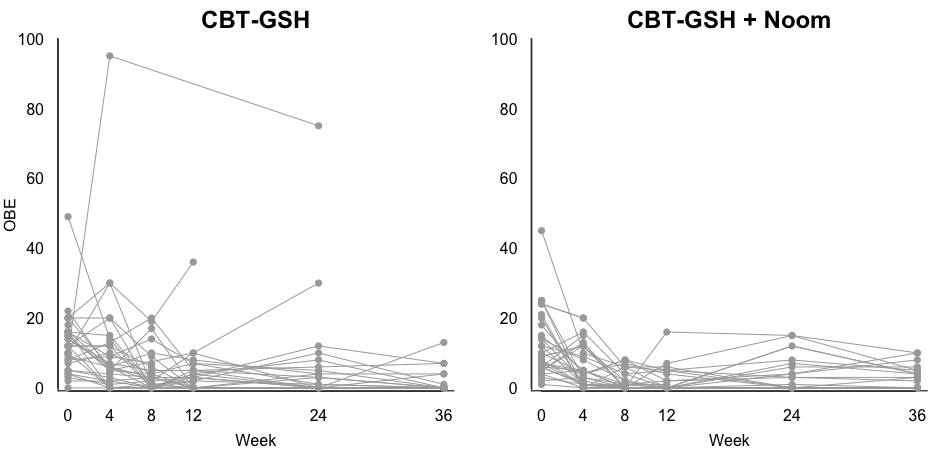
\includegraphics[width=\textwidth, height=\textheight, keepaspectratio]{Noom_paths.png}
\caption{\emph{Plots display OBEs over time for each individual in the CBT-GHS groups (left panel) and CBT-GHS + Noom group (right panel).}}
\end{figure}

Figure X displayes OBEs per week for each individual in both treatment conditions.  A few aspects of the data immediately stand out, which suggest that any model should account for individual-level effects and time-level effects, and should let treatment effects vary over time.  
\begin{itemize}
\item{The number of OBEs decreases over the course of the treatment for almost all subjects}
\item{The biggest decreases in OBEs appear to occur in the early stages of treatment}
\item{The primary sources of variation in OBE appear to be \emph{between people} and \emph{over time}.}
\end{itemize}

\newpage

\begin{figure}
\centering
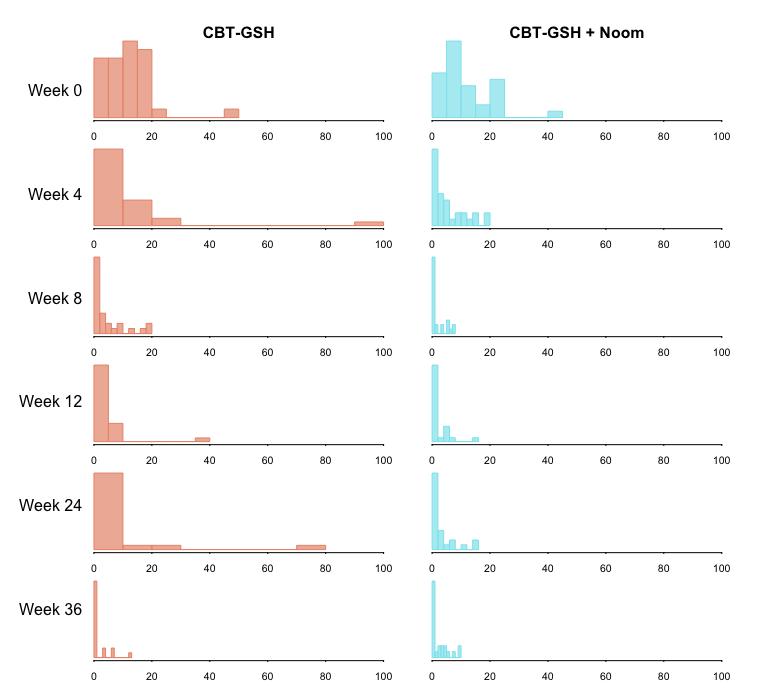
\includegraphics[width=\textwidth, height=\textheight, keepaspectratio]{noom_hist.png}
\caption{\emph{Histograms display the distribution of OBEs in each condition in each week.}}
\end{figure}

Figure Y displays the distribution of OBEs in each condition in each week.  We notice three characteristics of the data from these histograms.
\begin{enumerate}
\item{The distributions appear to condense around zero for both conditions over time} 
\item{The distributions in the CBT-GSH condition appear to have longer tails than those in the CBB-GSH+Noom condition}
\item{OBEs are count data; they must be nonnegative integers.}
\end{enumerate}
These three characteristics suggest that the appropriate model for OBEs is the Poisson distribution, because it is restricted to nonnegative integers and can concentrate its density around low numbers with a long tail.

\subsection{Model development}

\begin{table}[t]
\centering
\begin{tabular}{r l}
  Source of Prior Information &  \\ 
  \hline  \vspace{0.25em}
  Experimental Design & Outcome variable is nonnegative integers \\
  \vspace{0.25em}
  Literature & Effect size is close to zero \\
  Exploratory Data Analysis & There is variation in OBEs at the individual level \\
					  & There is variation in OBEs over time \\
                                            & Treatment effects may vary over time \\
    \hline
\end{tabular}
\caption{\emph{Sources of prior information.}}
\end{table}


We analyze RCTs by modeling the outcome of interest (in this case OBE) as a function of the treatment and all available pre-treatment covariates.  The coefficients associated with the treatment reveal the average treatment effects.  Inclusion of all available pre-treatment covariates accounts for variation in the outcome variable, decreasing uncertainly around treatment effects and providing the model with more predictive power.  We conduct \emph{intent-to-treat} analysis, meaning that our inferences will be based on initial treatment assignment, and will not account for mid-experiment dropouts.  
\\

The outcome variable is restricted to be nonnegative integers, so we fit a Poisson regression model, with hierarchies on individuals, time periods, and treatment effects.  For each individual in each time period, the number of OBEs follows a Poisson distribution, with a mean dependent on the characteristics of the individual and the time period.  

\begin{align}
OBE_{i,t} &\sim Poisson(\lambda_{i,t}) \\
\lambda_{i,t} &= exp(\alpha_i + \beta_t + \gamma_tT_i + X_i\theta) \\
T_i &=
    \begin{cases}
      0, & \text{if}\ CBT-GSH \\
      1, & \text{if}\ CBT-GSH + Noom \\
    \end{cases}
\end{align}

$\alpha$ is an individual-specific intercept, $\beta$ is a time-specific intercept, $\gamma$ is a time-specific treatment effect, $T$ is a treatment indicator, $X$ is a matrix of individual level covariates (age, sex, race, etc), and $\theta$ is a vector of effects. Subscripts $i = 1, ..., 66$ indicate individuals and subscripts $t = 0, 4, 8, 12, 24, 36$ indicate time periods.
\\

We believe that individual-level intercepts are simultaneously unique to the individual and common to the population; that is, each individual has their own baseline predilection to engage in eating disorder behavior, but their baseline predilections are not drastically different from each other.  We operationalize this concept by modeling all individual-level intercepts as coming from a common distribution, with \emph{hyperparameters} $\mu_{\alpha}$ and $\tau_{\alpha}$.
\begin{align}
\alpha_i \sim Normal(\mu_{\alpha}, \tau_{\alpha}) \ \forall \ i \in 1,...,66
\end{align} 

Similarly, we believe that time-specific treatment effects may be unique to each period but similar over time. We operationalize this concept by modeling all time-specific treatment effects $\gamma$ as coming from a common distribution, with \emph{hyperparameters} $\mu_{\gamma}$ and $\tau_{\gamma}$.
\begin{align}
\gamma_t \sim Normal(\mu_{\gamma}, \tau_{\gamma}) \ \forall \ t \in 0, 4, 8, 12, 24, 36
\end{align} 

$\mu_{\gamma}$ is the \emph{grand mean}, the overall treatment effect; $\tau_{\gamma}$ is the variation in treatment effects over time; and each individual $\gamma_t$ is a time-period specific treatment effect.  This approach has a natural smoothing effect: any extreme estimates of $\gamma_t$ will be partially-pooled back toward the grand mean $\mu_{\gamma}$.
\\

We assign the following prior and hyperprior distributions:
\begin{align}
\mu_{\alpha} &\sim Normal(5, 5) \\
\tau_{\alpha} &\sim Cauchy^+(0, 30) \\
\mu_{\gamma} &\sim Normal(0, 5) \\
\tau_{\gamma} &\sim Cauchy^+(0, 30) \\
\theta &\sim Normal(0, 1) \\
\end{align}

The normal distributions around the individual and treatment effects allow us to guide the model to the appropriate range of parameter values, but with wide enough variance (5 in each case) to let the model find its own way in that range.  Half cauchy priors on the variance parameters are weakly informative, with much of their mass around zero but gentle slopes in their tails, which have been shown to be effective prior distributions for variance parameters (Gelman, 2006).

\subsection{Model estimation}
We estimate this model with \emph{Hamilton Monte-Carlo} in Stan.  Model code is appended to this document.  We find that the model converges with four chains of 2000 iterations each (see table M).  

\subsection{Posterior predictive checking}

\begin{figure}
\centering
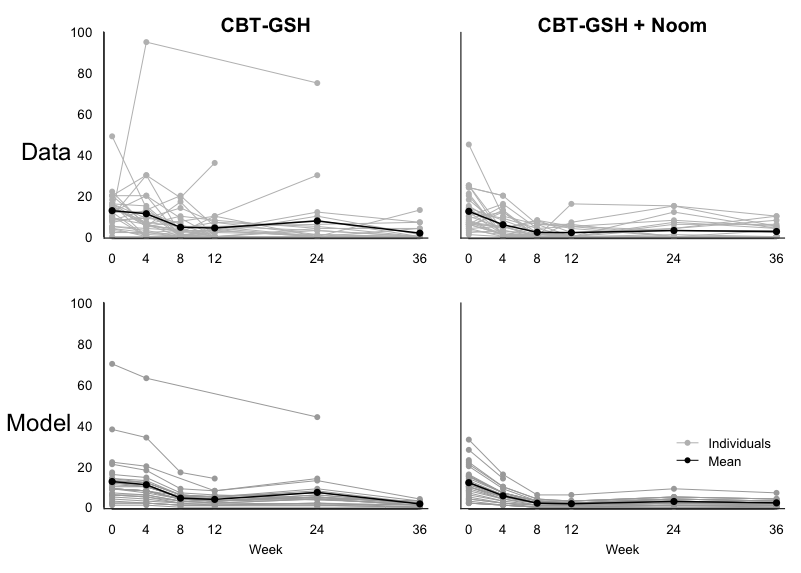
\includegraphics[width=\textwidth, height=\textheight, keepaspectratio]{ppc_sims.png}
\caption{\emph{Upper plots show OBEs in each period for each individual in both treatment group, with black lines representing means.  Lower plots show modeled OBEs for each individual in each treatment group, with black lines representing modeled means.  The model appears to be able to recover OBEs over time fairly well for both treatment conditions.}}
\end{figure}

Before using our model to make inferences about time-specific treatment effects, we check its fit by comparing model-simulated OBE to data OBE.  If model simulations do not track the data well, we may want to revisit our model's assumptions before trusting its inferences.  If the model's simulations recover patterns in the data, we are more inclined to trust its inferences.  
\\

Figure Q displays OBEs in each period for each individual in each treatment group, from raw data (upper plots) and model simulations (lowers plots).  Black lines display means for each.  This suggests that the model is broadly able to pick up on the key variables that determine OBE over time for the duration of this experiment.
\\

Another way to check the fit of the model is by comparing simulated data directly against the raw data.  Figure P shows this for both treatment conditions.  Simulated data for the Noom condition appears to better track the raw data than simulated data for the no Noom condition.  This is unsurprising, since the no Noom condition tended to have more outliers, which we would not expect (or want) our model to pick up perfectly from such a small sample.  
\\

\begin{figure}
\centering
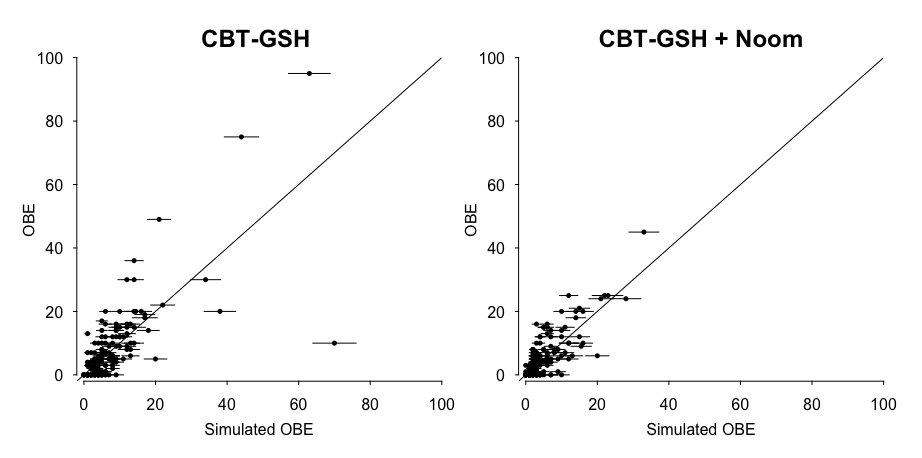
\includegraphics[width=\textwidth, height=\textheight, keepaspectratio]{obe_ppcs.png}
\caption{\emph{Plots display siulated OBEs to raw data for both treatment conditions.  Model simulations appear to match the raw data well, particularly for the Noom condition, which had fewer outliers.}}
\end{figure}

We conclude our model evaluations by mapping modeled density curves for each condition in each time period over the histograms in figure Y.  Figure BB shows that our model is able to broadly pick up on the patterns in the data over time and between treatment conditions.

\begin{figure}[h]
\centering
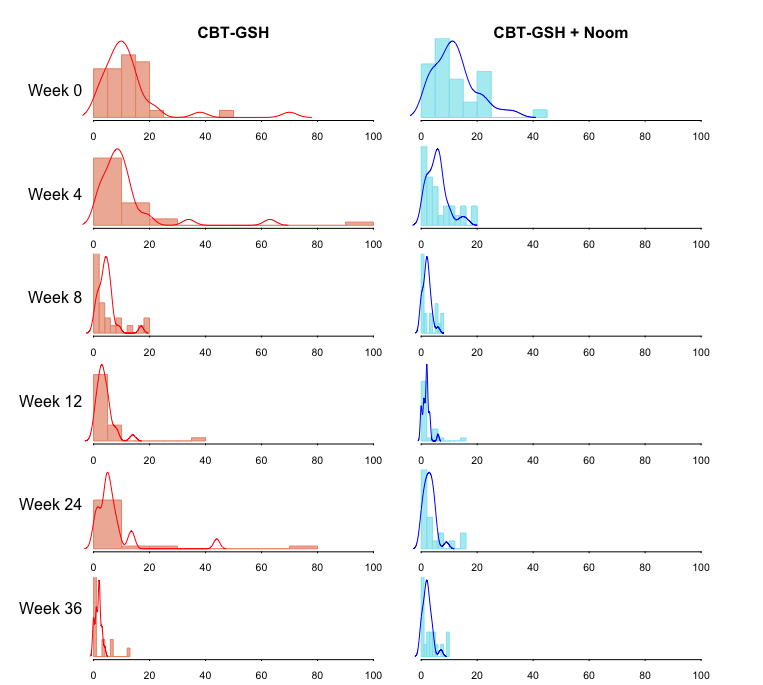
\includegraphics[width=\textwidth, height=\textheight, keepaspectratio]{ppc_hist_dens.png}
\caption{\emph{Histograms display the distribution of OBEs in each condition in each week.}}
\end{figure}

\subsection{Results}
Model results are displayed in table M.  Results suggest that using the Noom Monitor smartphone application during CBT-GSH may slightly decrease OBEs.  There some evidence that the treatment effect varies over time, with the Noom effect being slightly more pronounced during the later stages of therapy.
\\

Figure R displays modeled OBE for both treatment groups (upper plot) and smoothed treatment effects (lower plot).  In each measurement period, simulated OBE are higher for the No Noom condition than for the Noom condition, with some of the difference likely attributable to use of the Noom Monitor smartphone app.  

\begin{table}[t]
\centering
\begin{tabular}{r c c c c c}
  \hline
 & mean & 25\% & 50\% & 75\% \\ 
  \hline
  $\gamma_0$ & 0.18 & -0.45 & 0.15 & 0.78   \\ 
  $\gamma_4$ & -0.43 & -1.05 & -0.46 & 0.16   \\ 
  $\gamma_8$ & -0.70 & -1.33 & -0.71 & -0.10   \\  
  $\gamma_{12}$ & -0.65 & -1.28 & -0.68 & -0.04   \\  
  $\gamma_{24}$ & -0.72 & -1.34 & -0.75 & -0.11  \\  
  $\gamma_{36}$ & 0.21 & -0.42 & 0.19 & 0.82  \\ 
  \hline \hline
  $\mu_{\gamma}$ & -0.34 & -0.98 & -0.36 & 0.26  \\ 
  $\tau_{\gamma}$ & 0.64 & 0.43 & 0.56 & 0.77  \\ 
   \hline
\end{tabular}
\caption{\emph{Table displays model results for Noom effects in all six time periods and grand mean and variance parameters.}}
\end{table}


\begin{figure}[h]
\centering
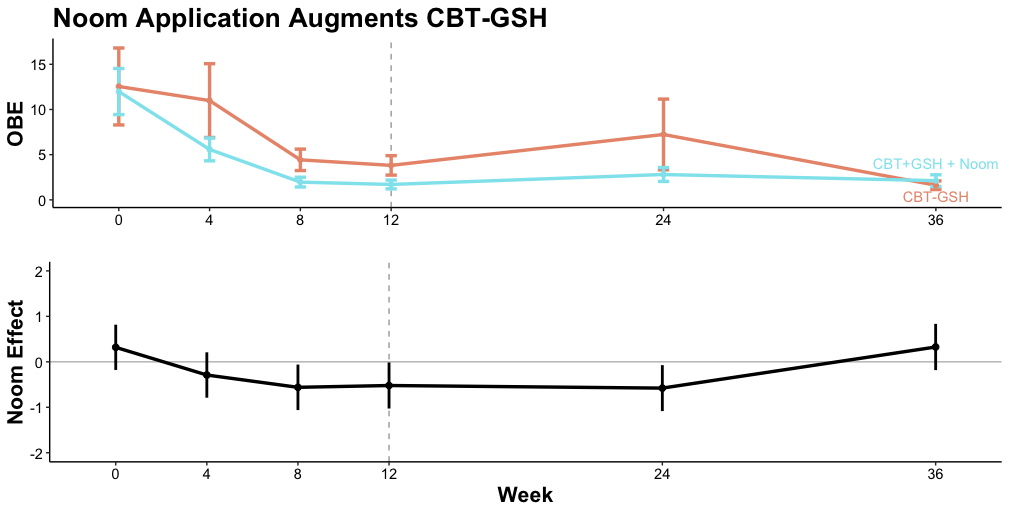
\includegraphics[width=\textwidth, height=\textheight, keepaspectratio]{noom_effect.png}
\caption{\emph{Upper plot displays modeled OBEs in each time period for the Noom (blue) and no Noom (orange) conditions with 95\% intervals.  Lower plot displays modeled treatment effects in each period,with 50\% intervals.}}
\end{figure}


\section{Conclusion}


\section{Appendix}


\end{document}